\chapter{Implementation}

In this chapter, we will go through our \emph{application generator}, explaining in detail how it works and how it is implemented from the inside. We will focus both on the \emph{platform} aspect and the \emph{framework} aspect. As for the \emph{platform} aspect, we will show how a non-developer can use the new \emph{platform} to generate and share Linked Data based applications. As for the \emph{framework} aspect, we will provide a potential developer with a step-by-step guide for how to implement a new \emph{visualizer}. As our generator is built on top of LinkedPipes Visualization, its official name is LinkedPipes Application Generator. For brevity, we will refer to it simply as to (our) \emph{application generator}. 

\section{Overview}

Before we dive into technical details, let us walk the reader through the \emph{application generator} features from a user perspective. We will start by describing a sample use case scenario and then we will continue with individual \emph{platform} features.

\subsection{Sample use case scenario}

In this scenario, we will utilize the D3.js Chord Visualizer and the Asylum Seekers 2015 data set. Both will be properly described later in a separate chapter dedicated to this particular visualizer. Let us say that our fictional user is a journalist writing an article on the refugee crisis. He comes across our \emph{application generator} and finds there the Asylum Seekers 2015 data set. The Figures \ref{fig:scenario-01-browse-data-sources} to \ref{fig:scenario-11-embedded-application} show step-by-step how the journalist can use our tool to create an interactive application and share it with his readers.

The actual mechanics of this visualizer will be explained later in the aforementioned separate chapter. Nevertheless, on a more general level this scenario nicely illustrates the principles that we suggested in the system proposal (Section \ref{sec:proposal:features}). The selected data set is automatically \emph{analyzed} and an appropriate visualization is offered to the user (Figure \ref{fig:scenario-02-discovery-result}). The configuration phase allows the user to work with the data and to affect the final shape of the application before it gets published. He can select for the visualization only the data he (or his audience) is interested in (Figure \ref{fig:scenario-05-search-graph}). He can even extend the data set itself with missing information (Figure \ref{fig:scenario-08-custom-label-editor}). Finally, the application can be easily shared using its public URL (Figure \ref{fig:scenario-09-published-app}).

What is also clear is that none of these steps require any advanced programming knowledge. The process is very \emph{non-developer friendly}. The only exception in this case is the preparation of the data set. Unfortunately, the original data are not available in RDF and the conversion has to be done by an expert. Nevertheless, once the data set is prepared and available in the \emph{application generator}, it can become a source for a large number of different applications.

\begin{figure}
	\centering
	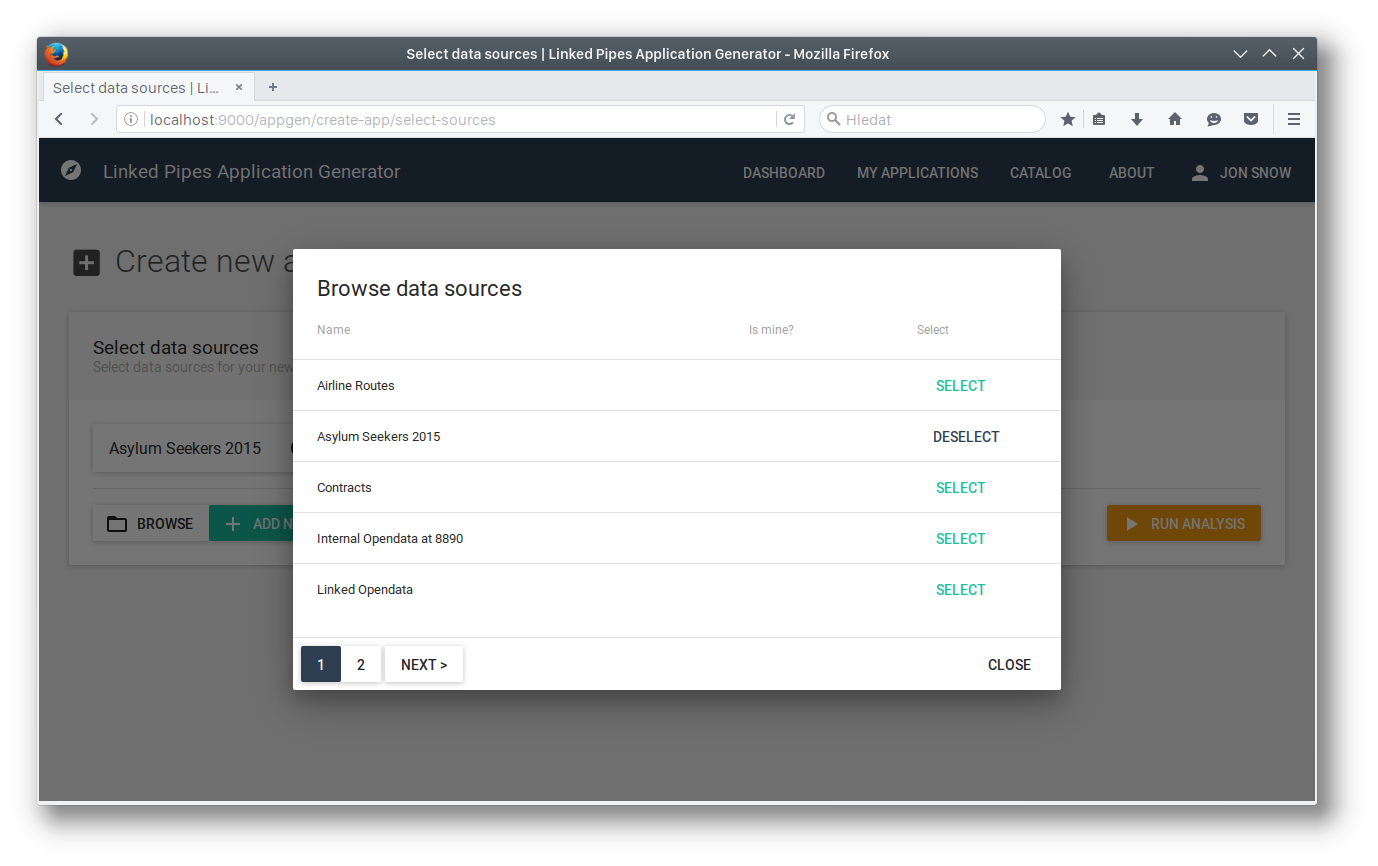
\includegraphics[width=145mm]{img/05_scenario_01_browse_data_sources.png}
	\caption{Use case scenario: Data source browser. The journalist selects the Asylum Seekers 2015 data set.}
	\label{fig:scenario-01-browse-data-sources}
\end{figure}

\begin{figure}
	\centering
	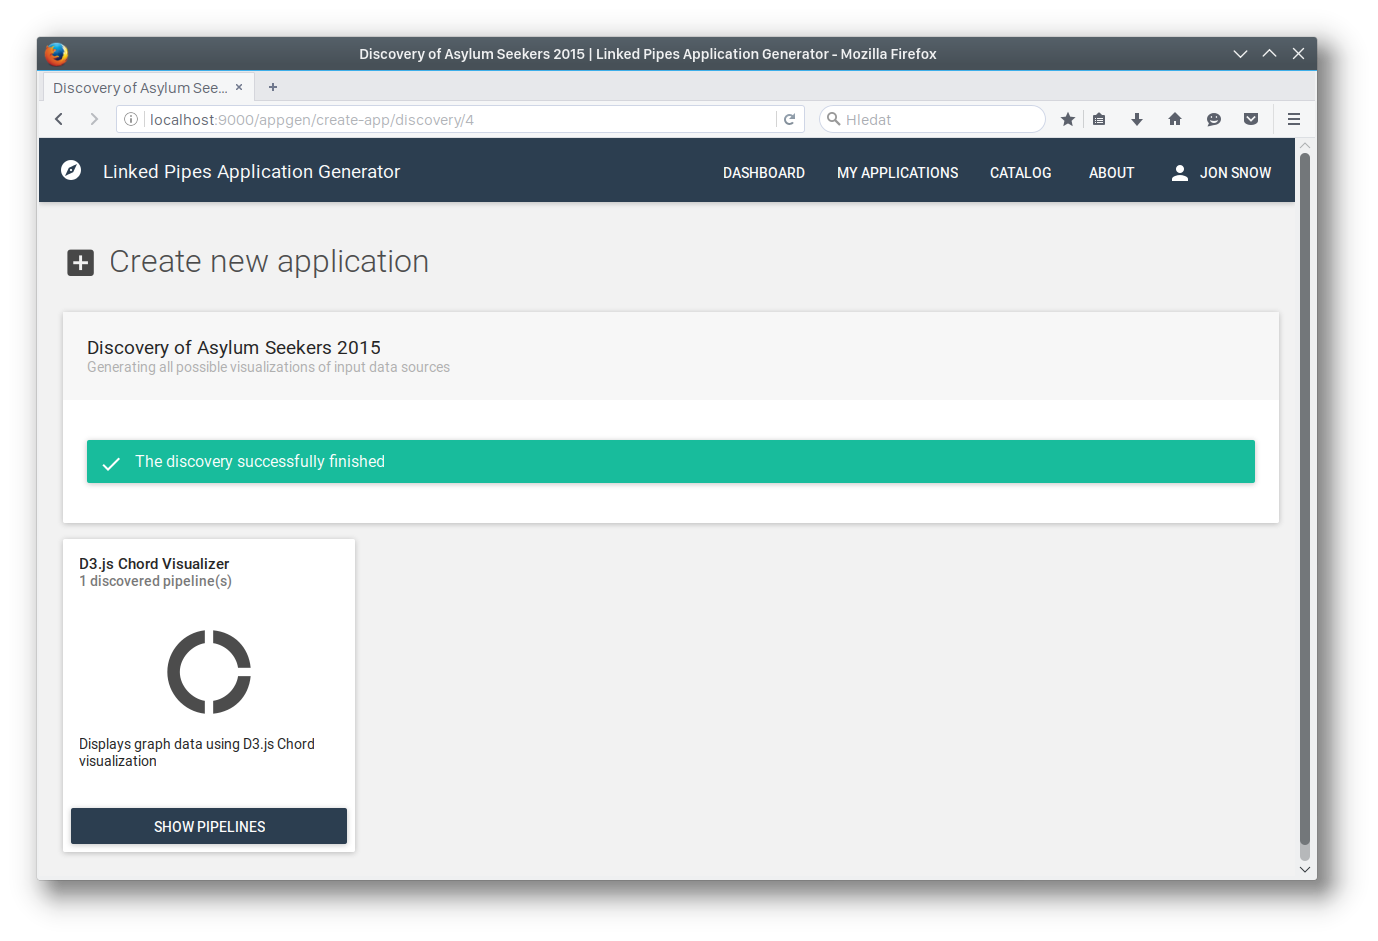
\includegraphics[width=145mm]{img/05_scenario_02_discovery_result.png}
	\caption{Use case scenario: Discovery result. The journalist can see that the Asylum Seekers 2015 data set can be visualized only using the D3.js Chord Visualizer. He runs the one discovered LDVM \emph{pipeline} that ends with this particular LDVM \emph{visualizer component}.}
	\label{fig:scenario-02-discovery-result}
\end{figure}

\begin{figure}
	\centering
	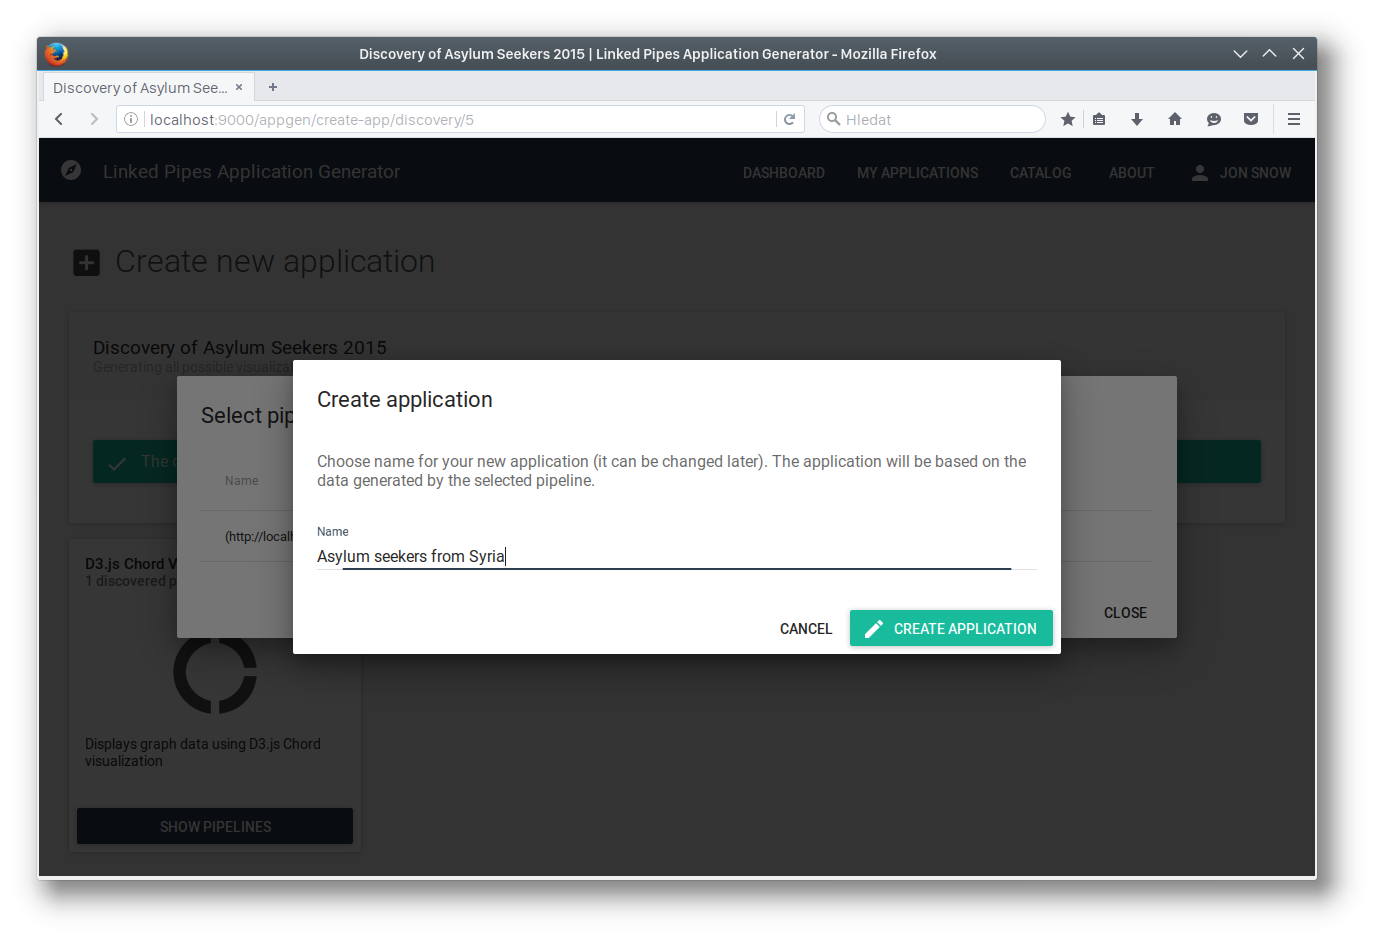
\includegraphics[width=145mm]{img/05_scenario_03_create_application.png}
	\caption{Use case scenario: Create application dialog. When the \emph{pipeline evaluation} is done, the user can proceed by creating an application.}
	\label{fig:scenario-03-create-application}
\end{figure}

\begin{figure}
	\centering
	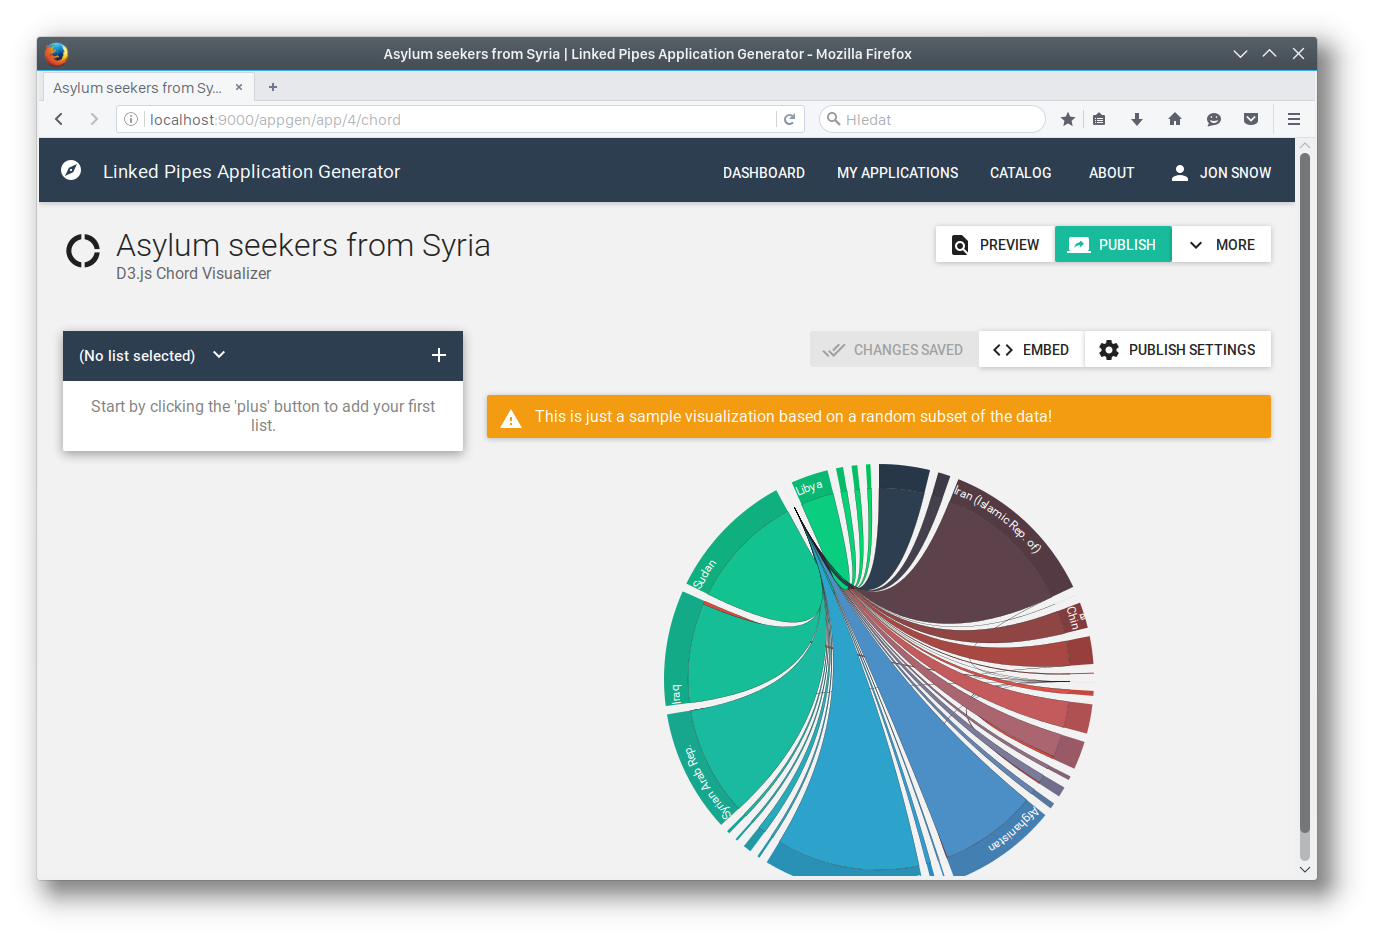
\includegraphics[width=145mm]{img/05_scenario_04_graph_sample.png}
	\caption{Use case scenario: Configurator of D3.js Chord Visualizer. Immediately after the application is created, the journalist is presented with a random sample visualization of the data.}
	\label{fig:scenario-04-graph-sample}
\end{figure}

\begin{figure}
	\centering
	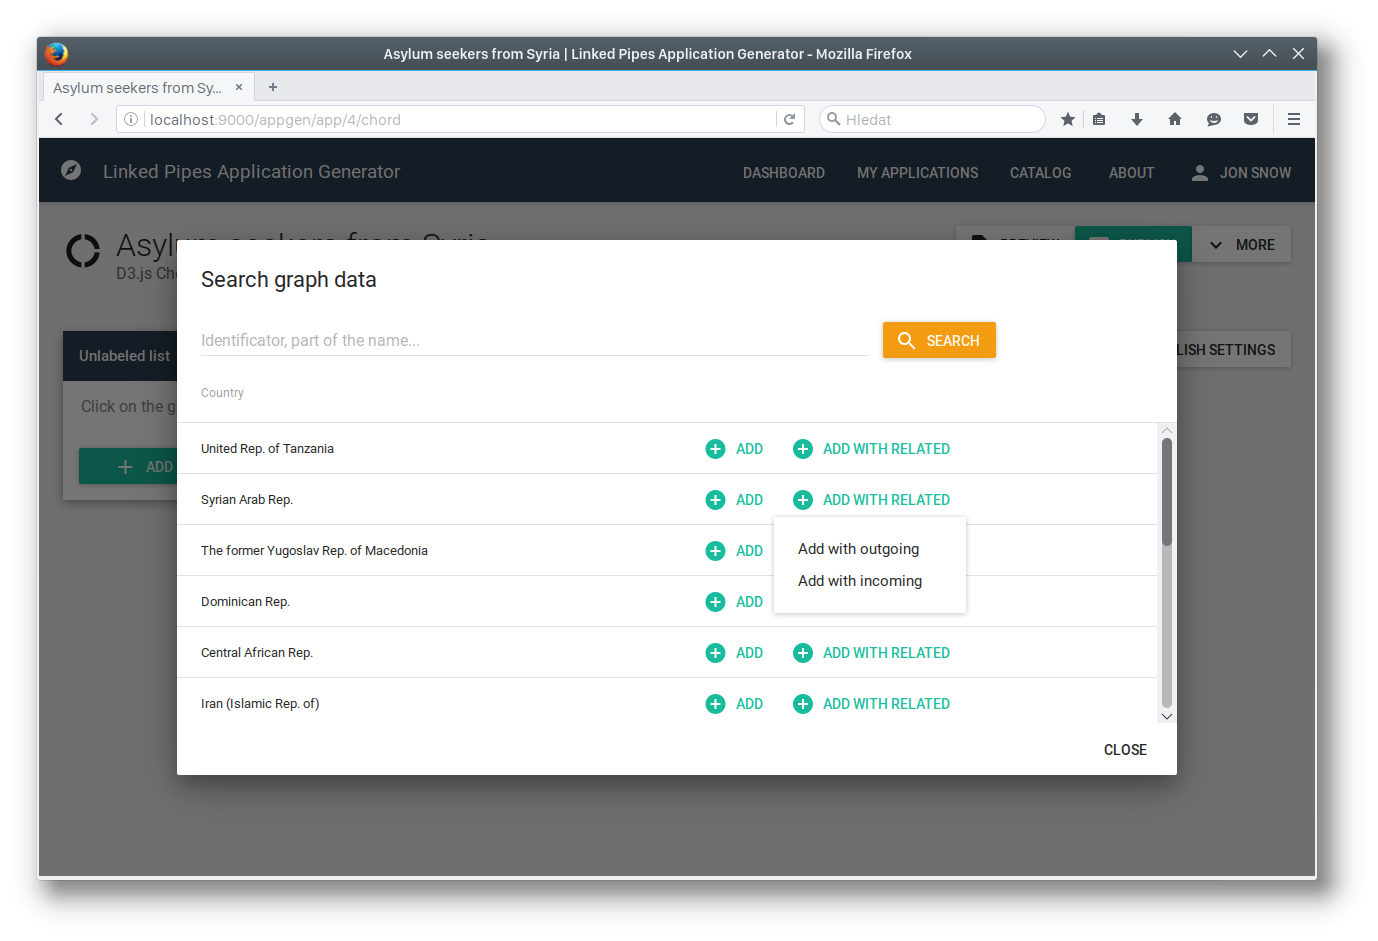
\includegraphics[width=145mm]{img/05_scenario_05_search_graph}
	\caption{Use case scenario: Search dialog. The journalist wants to create a visualization of asylum seekers coming from Syria. He uses the search feature to find Syria in the data set and adds it together with all target countries to the visualization \emph{list}.}
	\label{fig:scenario-05-search-graph}
\end{figure}

\begin{figure}
	\centering
	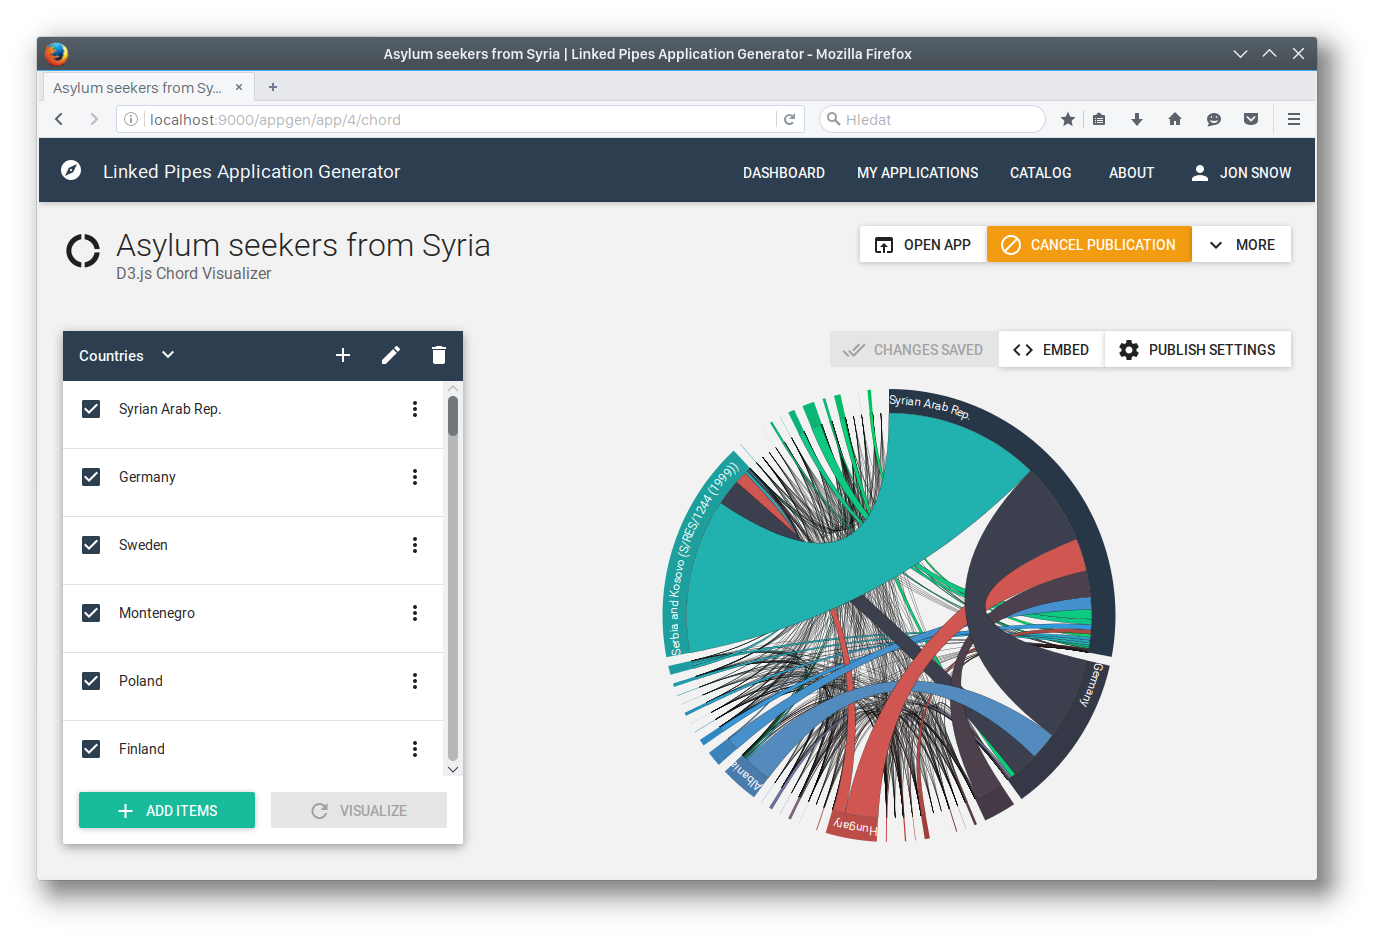
\includegraphics[width=145mm]{img/05_scenario_06_ready_application}
	\caption{Use case scenario: Visualization of selected countries. The journalist is now presented with the chord diagram of the countries he added into the \emph{list}.}
	\label{fig:scenario-06-ready application}
\end{figure}

\begin{figure}
	\centering
	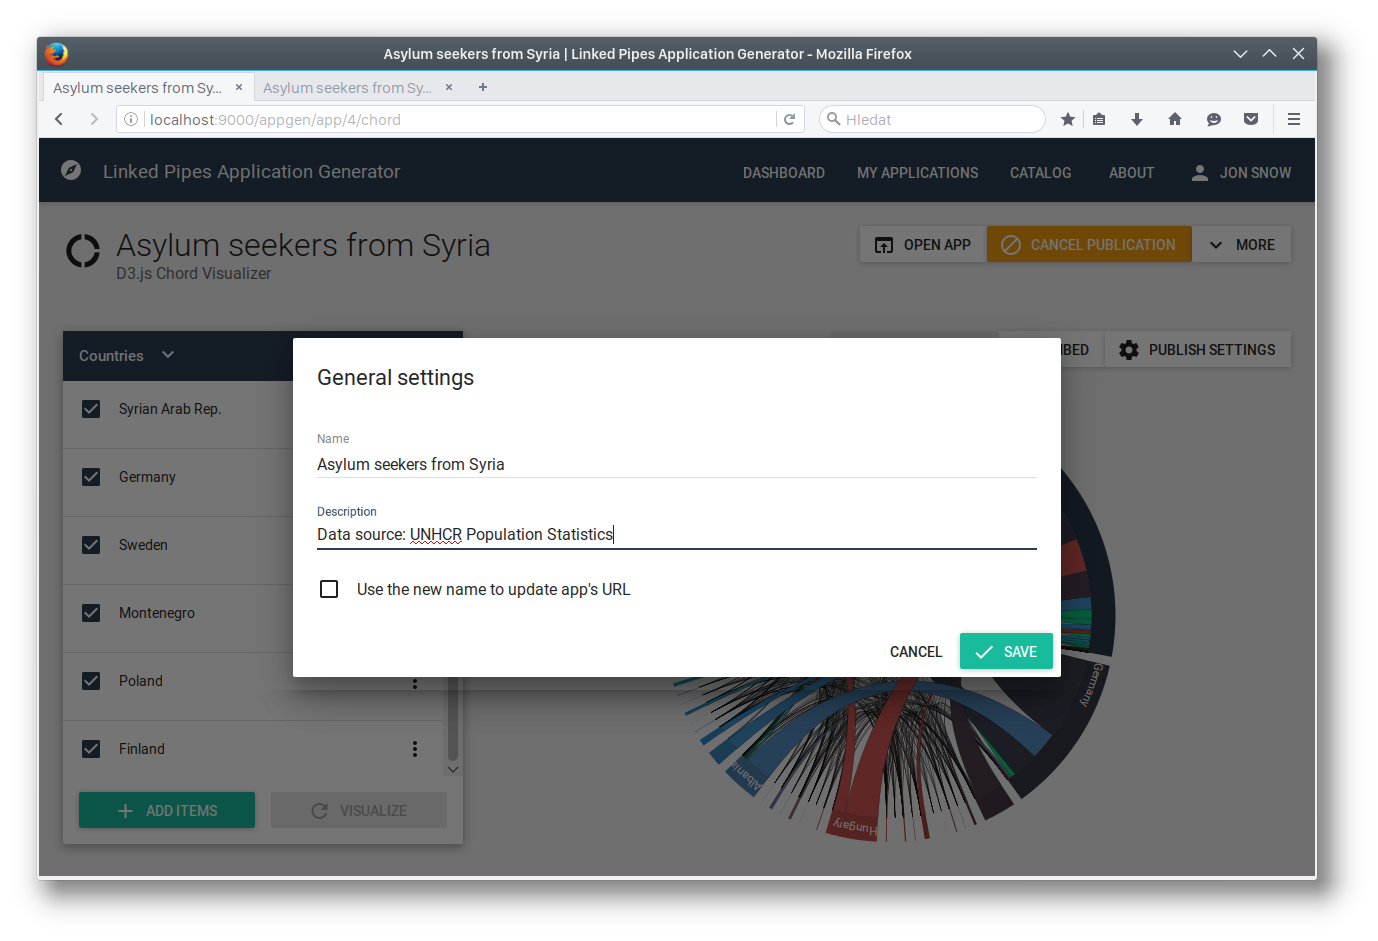
\includegraphics[width=145mm]{img/05_scenario_07_general_settings}
	\caption{Use case scenario: General application settings. The journalist can also provide the application description (in this case he uses it to explicitly mention the source of the data).}
	\label{fig:scenario-07-general-settings}
\end{figure}

\begin{figure}
	\centering
	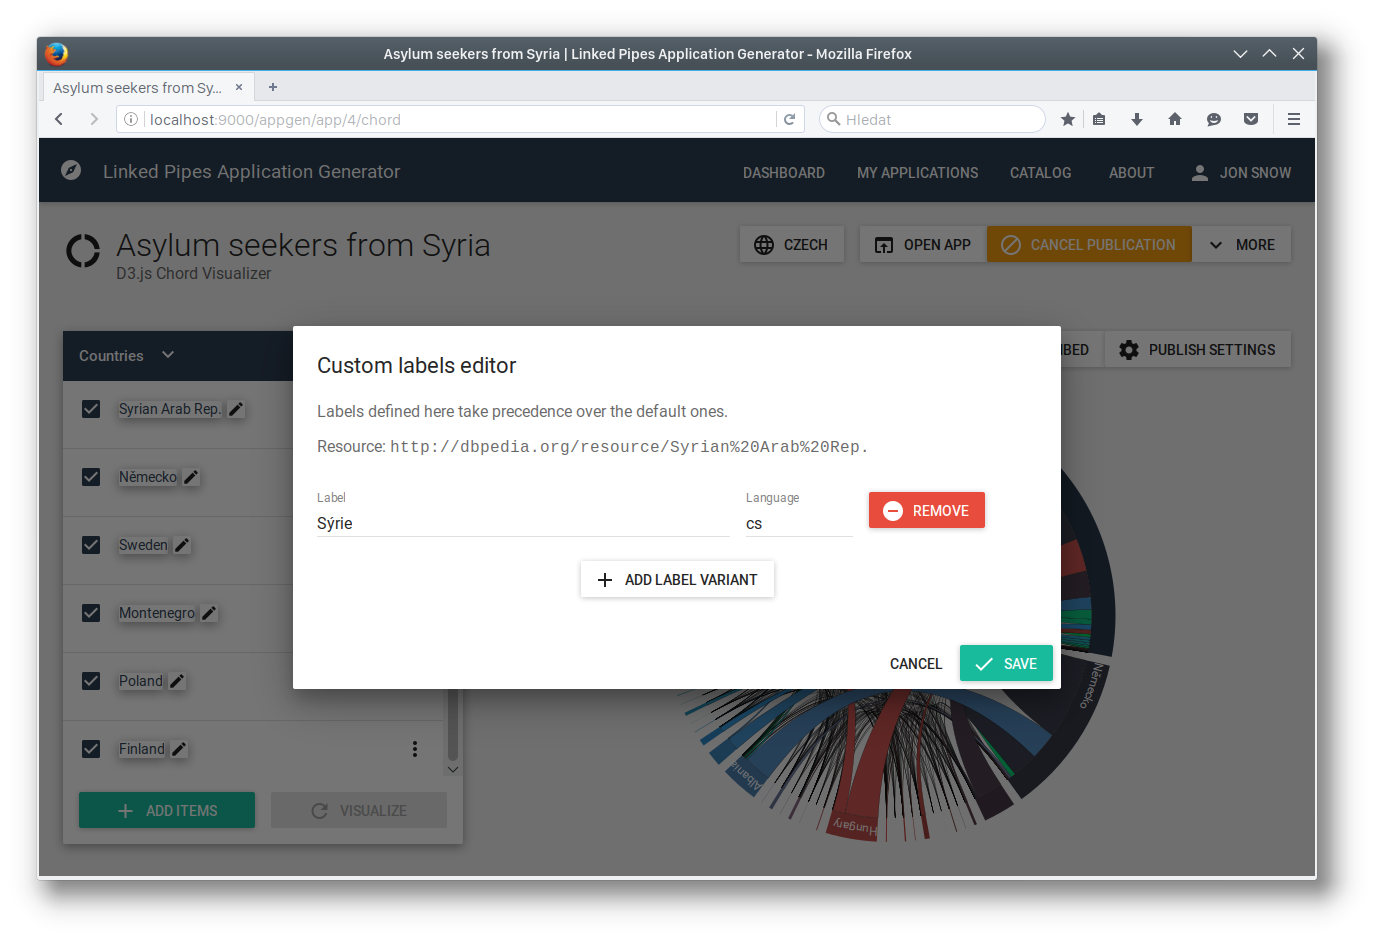
\includegraphics[width=145mm]{img/05_scenario_08_custom_label_editor}
	\caption{Use case scenario: Custom labels editor. The journalist is targeting Czech audience but the country names in the data set are in English. The configurator lets the journalist provide his own names that will override the default ones. }
	\label{fig:scenario-08-custom-label-editor}
\end{figure}

\begin{figure}
	\centering
	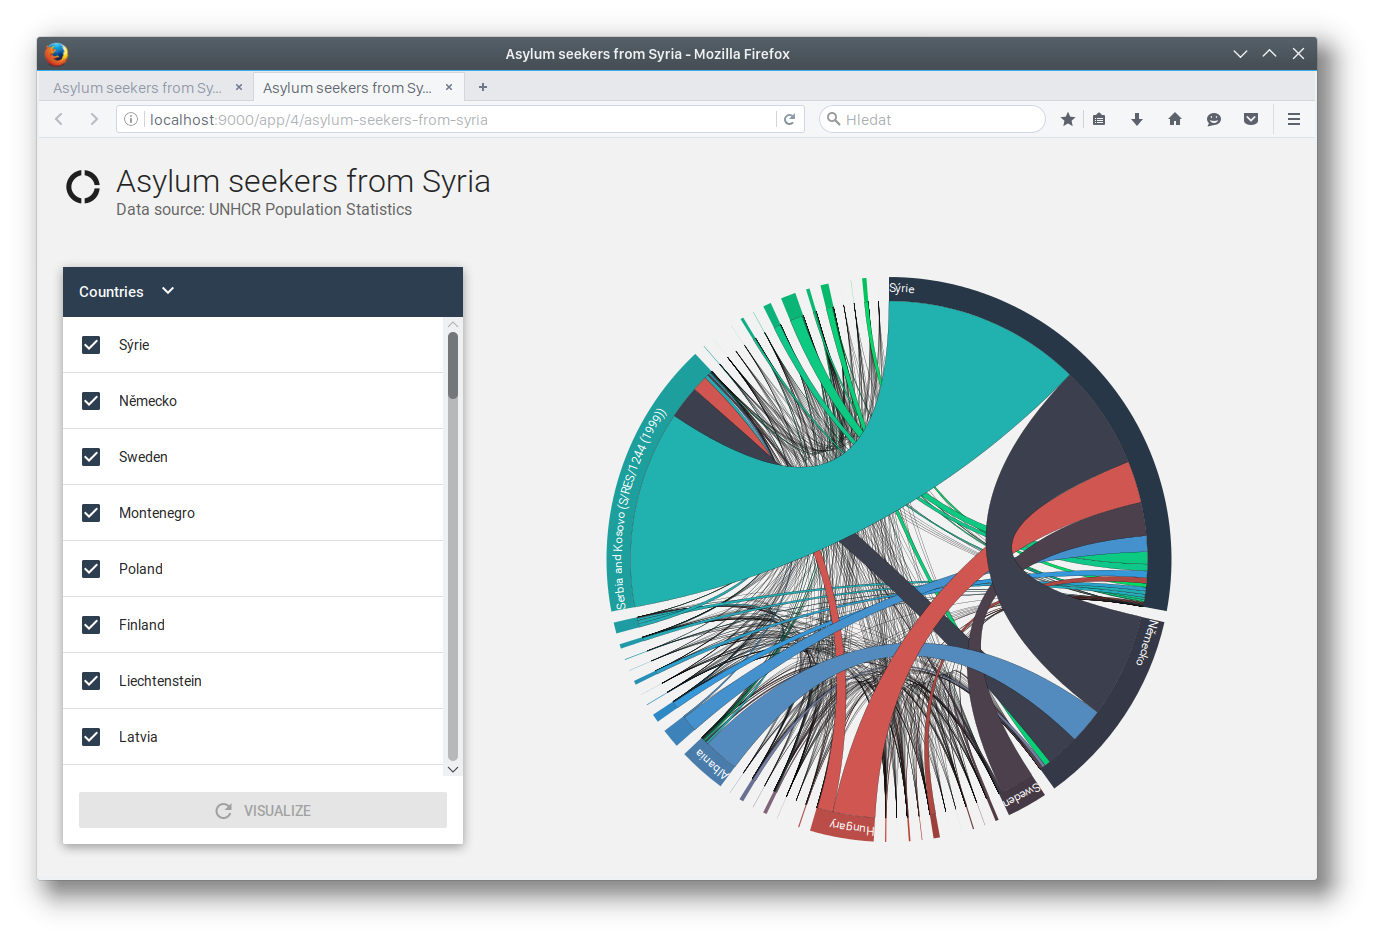
\includegraphics[width=145mm]{img/05_scenario_09_published_app}
	\caption{Use case scenario: Published application. This is what the journalist's readers will see when the application gets published. Using the menu on the side, the users can switch on/off individual countries in the chord diagram.}
    \label{fig:scenario-09-published-app}
\end{figure}

\begin{figure}
	\centering
	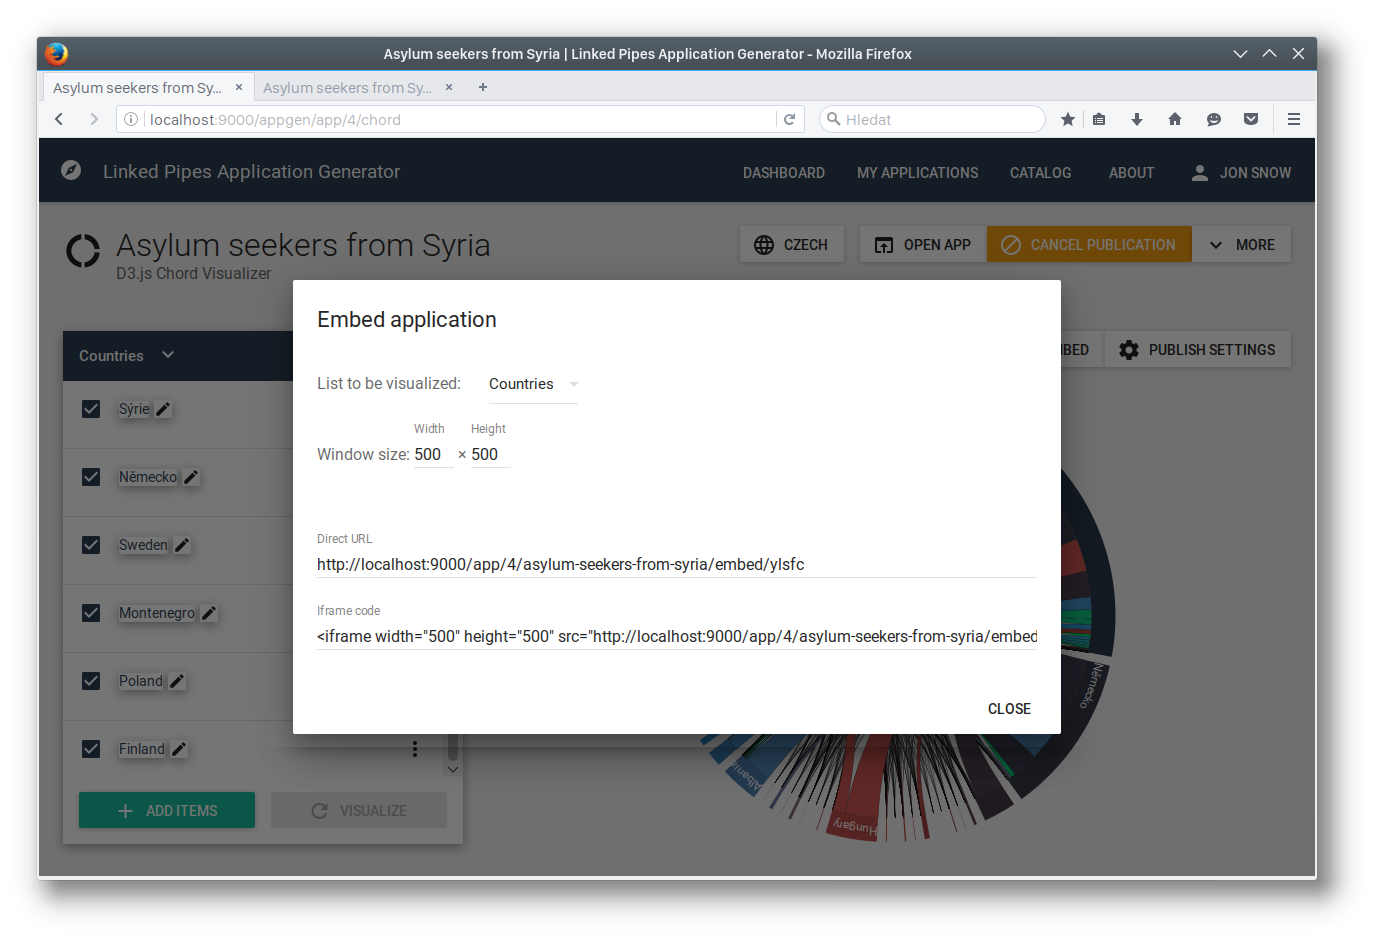
\includegraphics[width=145mm]{img/05_scenario_10_embed_application}
	\caption{Use case scenario: Embed application dialog. The journalist may decide to embed the chord diagram directly into his article.}
    \label{fig:scenario-10-embed-application}
\end{figure}

\begin{figure}
	\centering
	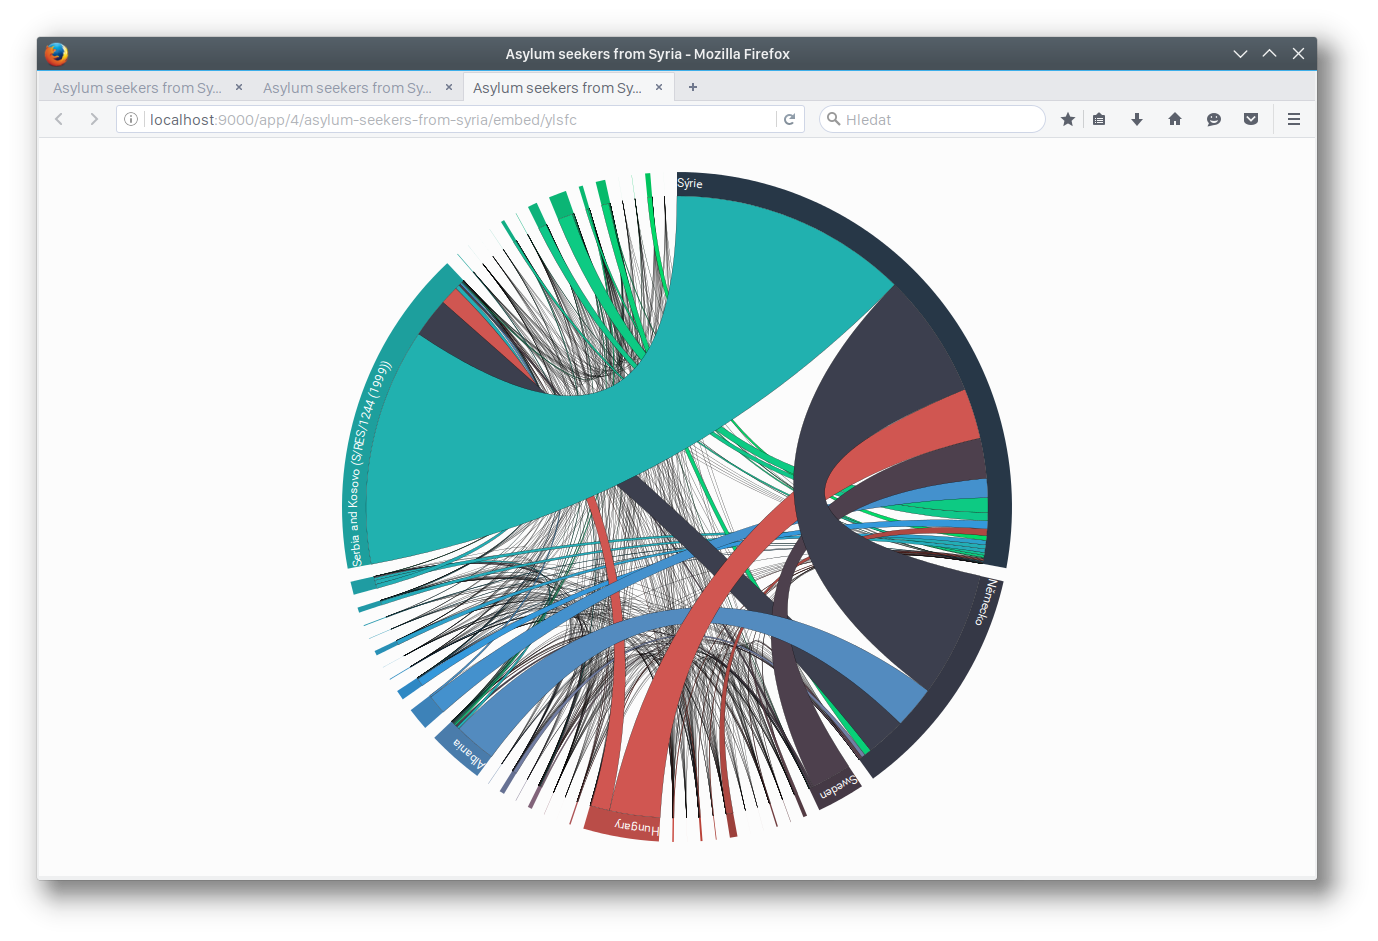
\includegraphics[width=145mm]{img/05_scenario_11_embedded_application}
	\caption{Use case scenario: Embedded application. In this form, stripped from all controls to the bare visualization, it is perfect for direct embedding into web pages.}
    \label{fig:scenario-11-embedded-application}
\end{figure}


\subsection{Users}

Everyone who wants to use our \emph{application generator} needs to create an account first. At this moment, a user can either create a standard local account protected by a password or he can log in with his Google account. No other providers are currently supported. As the user works with the \emph{application generator}, all his applications, data sources and discoveries are linked to his account and no one else can access it. E.g. an application can be configured only by its owner and before it is published, only the owner can view it.

One exception are \emph{administrator} accounts which work similarly to root users known from Unix systems. Such users can access and update any applications, data sources or discoveries in the system. The first user to register in our \emph{application generator} automatically becomes an administrator. The others have to be manually appointed (which is currently not possible through the user interface and has to be done by directly updating the database record).

\begin{figure}
	\centering
	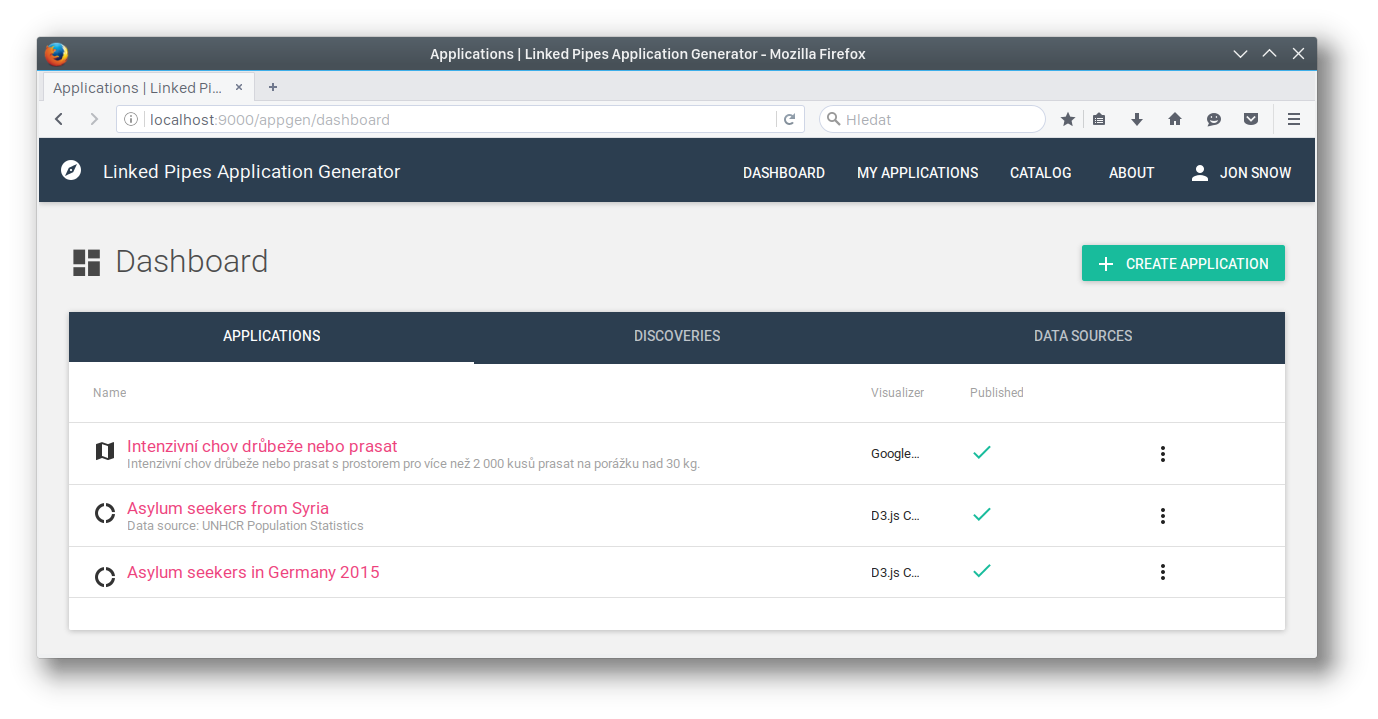
\includegraphics[width=145mm]{img/05_dashboard}
	\caption{User dashboard showing the overview of applications, discoveries and data sources}
    \label{fig:dashboard}
\end{figure}

\subsection{Data sources}

Our  approach to data sources is slightly different to LinkedPipes Visualization. In LinkedPipes Visualization, the user starts by providing the data source (may it be the SPARQL endpoint URL or a *.ttl file with serialized RDF data) and he has to do it every single time he wants to create a visualization. In our \emph{application generator}, we focused more on the possibility to re-use and share the data sets. So the user has to start by adding a data source to the generator, giving it a common name and only then he is allowed to select it for visualization. 

If we just have a new data set and want to get to a visualization quickly, the approach of LinkedPipes Visualization is faster. But once we want to re-use that data set, our approach wins over. 

That is not the only advantage. In our \emph{application generator}, we distinguish between public and private data sources. Private data sources are seen only by their owner (it should be mentioned that they are just hidden by the user interface, they are not actively protected from being used by other users). Public data sources, on the other hand, ale openly available for anyone and can be selected in the data source browser (Figure \ref{fig:scenario-01-browse-data-sources}). Any user can decide to make any of his data sources public. The idea is that one user (a data expert) might prepare the data set and another might use it to generate an application.

This approach introduces another level of abstraction. The user generating an application does not have to know what RDF or a SPARQL endpoint is, i.e, he is separated from the technical details. He can simply select the data source he is interested in from the browser and use it.

\subsection{Pipeline discovery}

The \emph{application generator} runs the underlying LDVM \emph{discovery} algorithm on the selected data sources. The \emph{discovery} returns all possible LDVM \emph{pipelines} that lead to a visualization, i.e., they end with a \emph{visualizer component}. Multiple \emph{pipelines} might use the same \emph{visualizer component} (they might use different \emph{analyzers} and \emph{visualizer transformers} along the way to get the input data compatible with this particular visualizer). Unfortunately, we are not able to give the user any detailed information about how the data produced by a \emph{pipeline} will look like. The only way to find out is to actually run the \emph{pipeline} and create an application from it. If the data do not make sense or are not what the user expects, he can try another one.

The user can watch the \emph{discovery} algorithm progress on a dedicated screen that shows the current \emph{discovery} status and also the list of \emph{pipelines} that have been discovered so far (Figure \ref{fig:scenario-02-discovery-result}). The \emph{pipelines} are grouped by \emph{visualizers}. As the algorithm may take some time, the user can leave the screen and come back later. It is accessible even after the \emph{discovery} algorithm finishes. The list of all discoveries can be found on the dashboard \ref{fig:dashboard}.

Note that not all \emph{visualizer} are supported by our \emph{application generator} (i.e., the corresponding \emph{plugin} is missing). For example, LinkedPipes Visualization contains a \emph{visualizer} for statistical data described using Data Cube Vocabulary \cite{datacube_vocabulary}. If the appropriate LDVM \emph{component} is registered in our \emph{application generator}, the \emph{discovery} algorithm will return \emph{pipelines} that use this \emph{component}. However, those will not be offered to the user.

\subsection{Application configuration}

The configuration phase is the core feature of the \emph{application generator} which differentiates it from the LinkedPipes Visualization. The application configuration involves both tasks that are common for all applications (e.g. publishing, deleting, updating description etc.) and that are \emph{visualizer} specific. As you can see on the Figure \ref{fig:configurator}, the \emph{configurator} interface follows this principle. It is divided into the common area and the area which is controlled by a particular \emph{visualizer} plugin (see Figure \ref{fig:google_maps_visualizer} of how a different \emph{visualizer} adapts to the universal configurator interface). 

\begin{figure}
	\centering
	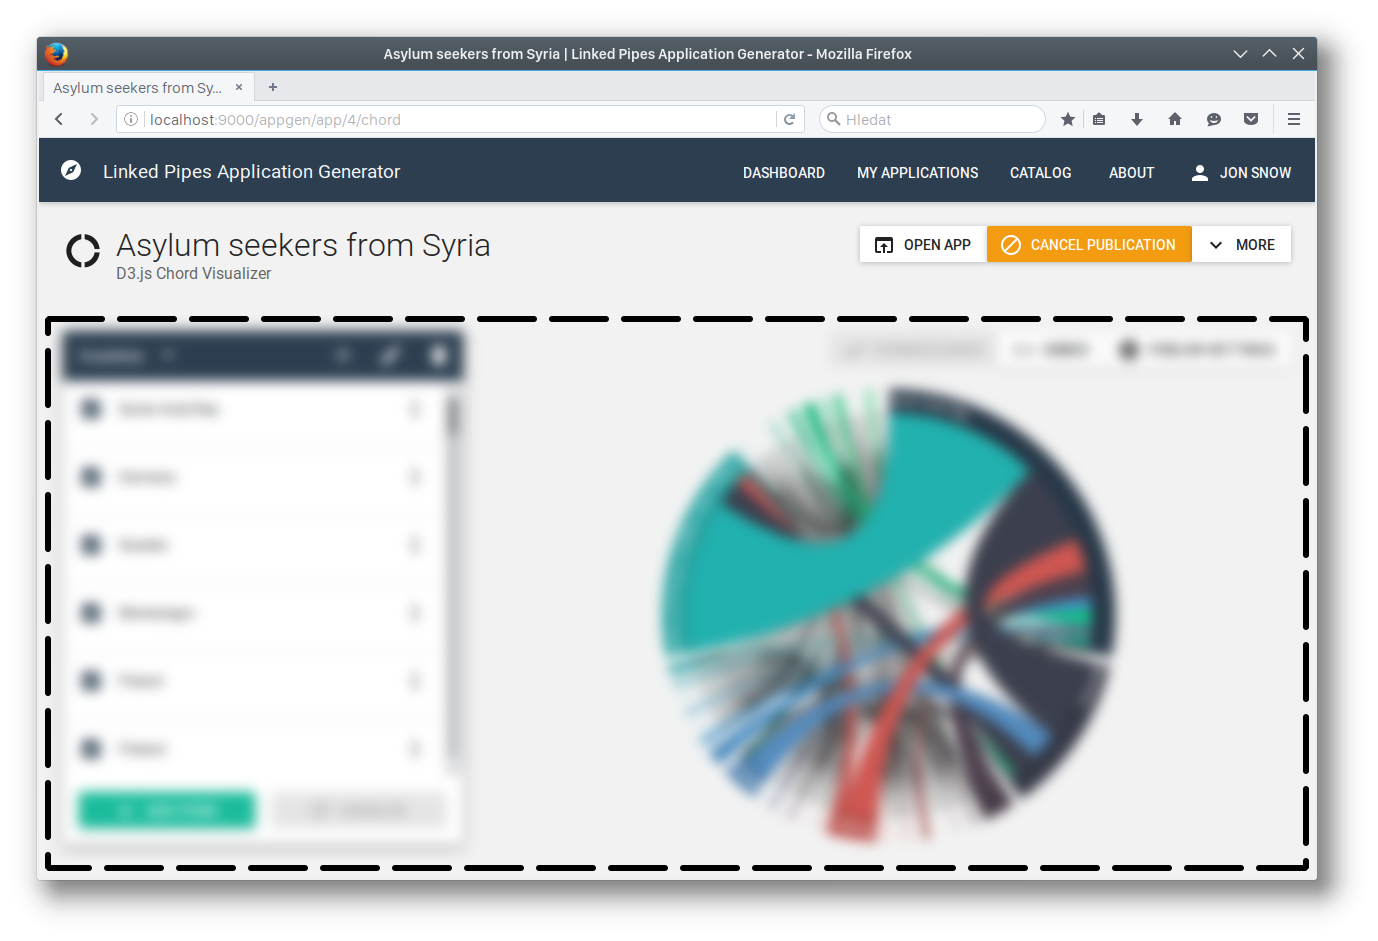
\includegraphics[width=145mm]{img/05_configurator.png}
	\caption{The configurator interface. The blurred out part is controlled by the current visualizer whereas the rest is identical for all visualizers. It contains the common functionality (e.g. the "More" button in the upper right corner shows a menu allowing the user to delete the application or change the application name and description).}
    \label{fig:configurator}
\end{figure}

\begin{figure}
	\centering
	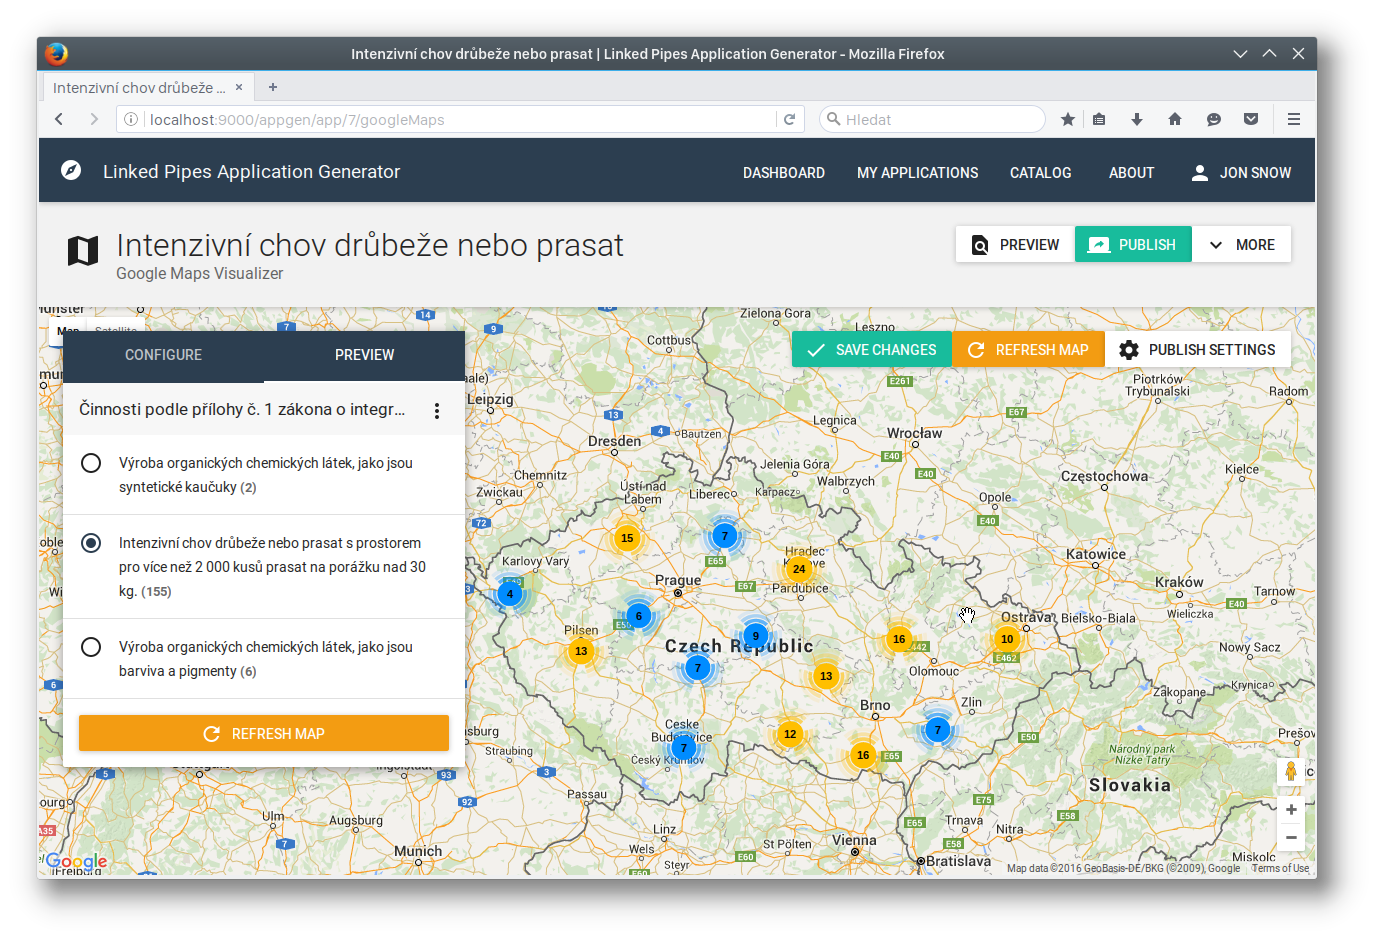
\includegraphics[width=145mm]{img/05_google_maps_visualizer.png}
	\caption{The configurator interface of the Google Maps Visualizer.}
    \label{fig:google_maps_visualizer}
\end{figure}

\subsection{Publishing applications}

When the user is happy with how the application looks, he can publish it by hitting the green "Publish button" (as seen for example on the Figure \ref{fig:scenario-04-graph-sample} in the upper right corner). The application then becomes accessible on a public URL which is generated from the application ID (internal numeric identificator) and its name. The \emph{application generator} at this moment does not offer any fine grained control of who gets to access the application. It is either public or not. Once it is published, it also becomes part of the public application catalog (Figure \ref{fig:catalog}).

\begin{figure}
	\centering
	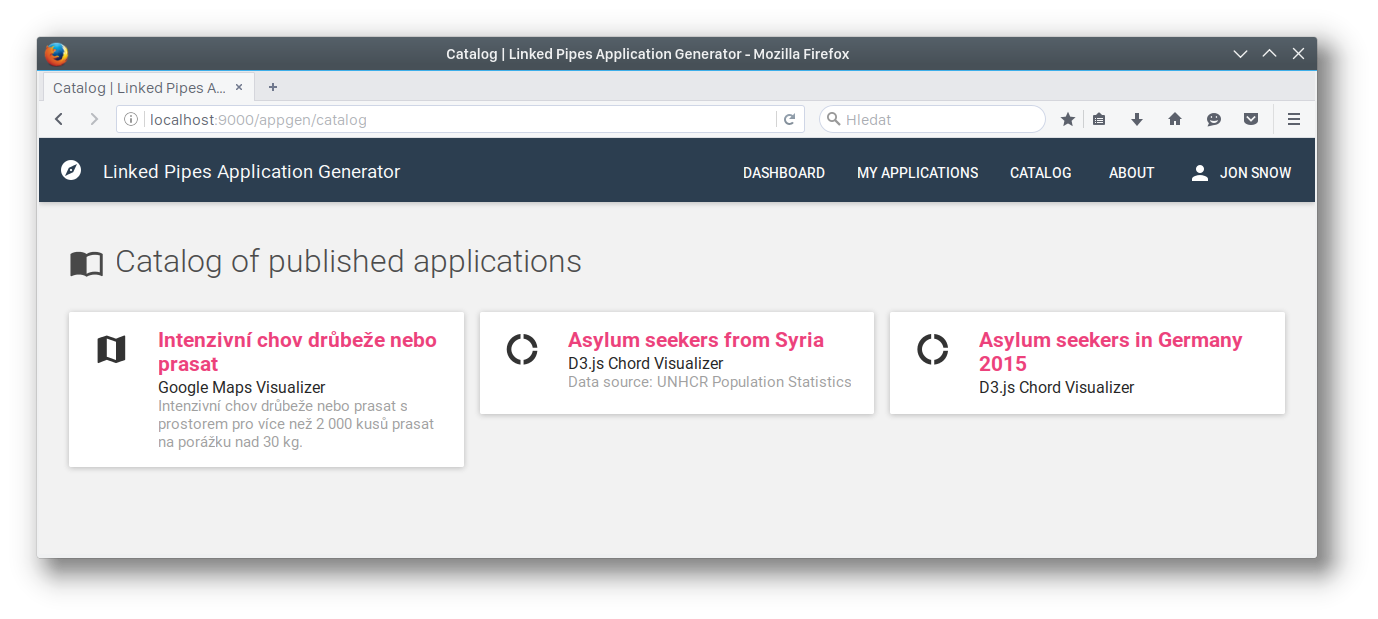
\includegraphics[width=145mm]{img/05_catalog}
	\caption{Catalog of published applications.}
    \label{fig:catalog}
\end{figure}

Some \emph{visualizers} offer the option to publish the application in an embed mode. That means that the application's interface is adapted so that it can be inserted for example into an external online article. The interface is usually significantly reduced and stripped from unimportant  control elements. This functionality is not considered common for all \emph{visualizers}  as each \emph{visualizer} can approach it differently. For example, the D3.js Chord Visualizer we used in this section allows the user to create multiple chord diagrams within a single application. Each of these diagrams can be exported separately in the embed mode (a unique URL is generated for each diagram under which the diagram is accessible). See Figure \ref{fig:scenario-10-embed-application}. Clearly, this functionality is specific for D3.js Chord Visualizer.

\section{General architecture}

We decided that we build our \emph{application generator} on top of LinkedPipes Visualization (Section \ref{sec:system_proposal:integration}). We already described the architecture of this tool (Section \ref{sec:linkedpipes:architecture} and especially Figure \ref{fig:linked-pipes-visualization-architecture}). We will now explain how we integrated the \emph{application generator} into LinkedPipes Visualization. You will get the overall idea by referring to Figure \ref{fig:application-generator-architecture}.

\begin{figure}
	\centering
	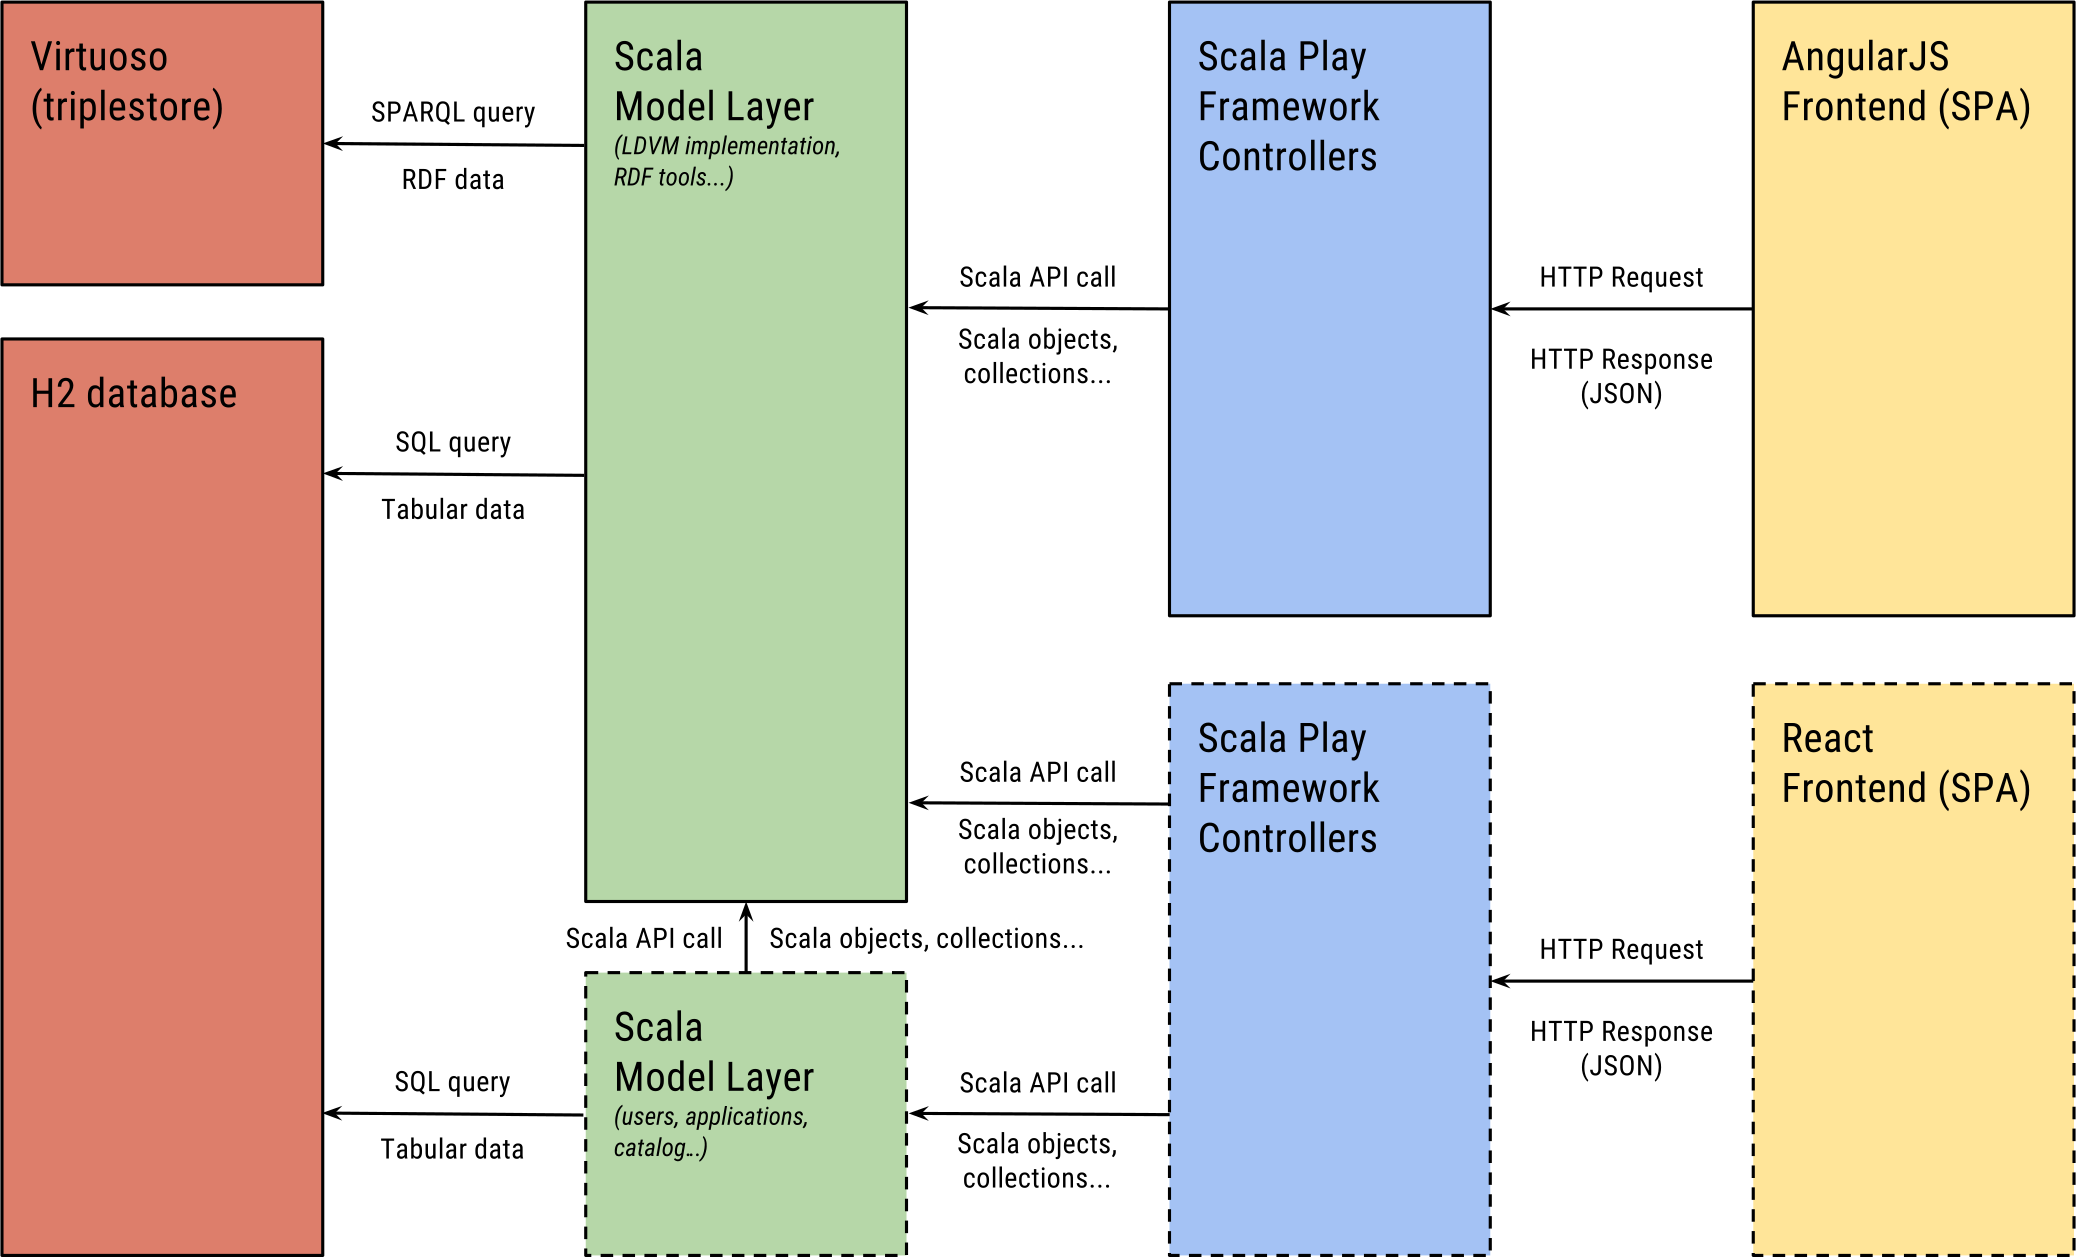
\includegraphics[width=140mm]{img/05_application_generator_architecture.png}
	\caption{Application Generator Architecture. Blocks with solid borders are part of the original LinkedPipes Visualization, blocks with dashed borders are newly implemented parts of the \emph{application generator}.} 
	\label{fig:application-generator-architecture}
\end{figure}

The \emph{application generator} is part of the original LinkedPipes Visualization code base. We made this decision after consulting the authors of LinkedPipes Visualization. From the software architectonic perspective, it is probably not the cleanest approach, but it significantly sped up our work. The original code base contained many solutions and APIs that we could immediately use (for example the LDVM implementation API, various RDF tools etc.). Nevertheless, even though both tools live in the same code base, we made sure to keep them as separated as possible (Figure \ref{fig:application-generator-architecture} shows that clearly). So if we decided in the future to separate both tools or for example replace the underlying LDVM implementation, it should not be impossible.

\subsection{Frontend}

The \emph{application generator} frontend is completely new and independent on the original frontend. The original frontend already contained some work that we could at first glance use (e.g. existing \emph{visualizer} plugins). Unfortunately, couple of problems prevented us from doing so. Firstly, the AngularJS frontend was created just to showcase the capabilities of the underlying LVDM implementation. For this reason, its code was in a rather poor state with no documentation. Clearly, it would take us lots of time to get familiar with it. Secondly, this code was not written with certain features (like for example user support) in mind. Thirdly, our \emph{visualizers} (with the separated \emph{configurator} and \emph{application} interfaces) work very differently compared to the \emph{visualizers} of LinkedPipes Visualization. Having these three reasons in mind, we came to the conclusion that we would have to rewrite a major portion of the original code anyway and therefore we decided to start from the scratch. We also decided to go with a different development stack (we replaced AngularJS with React and related tools) which we believed would fit our needs better. 

As a result, there are two existing user interfaces that live within the same application next to each other. The original LinkedPipes Visualization interface is accessible from the home page (the \texttt{/} URL). Our \emph{application generator} can be found at \texttt{/appgen} and individual published applications live at \emph{/app}.

\subsection{Controllers}

The vast majority of controllers in both LinkedPipes Visualization and the \emph{application generator} handle the asynchronous HTTP requests coming from the frontend (the only exception are the controllers handling the initialization of the SPAs). The role of a controller in this typical case is just to translate the HTTP request into an API call to the \emph{Model} layer and send the response back. All controllers together define a public remote API interface.

Even though we could re-use some of the methods available from the LinkedPipes Visualization controllers (e.g. those for controlling the \emph{discovery} algorithm), we decided not to do that to avoid hidden dependencies between the frontend and the backend. Dependencies within the Scala code base (for example between the \emph{Controller} layer and the \emph{Model} layer) are easy the discover. If they break, the code will not compile. That is not true for the remote API. Therefore the \emph{application generator} frontend strictly uses only those remote API methods that are handled by the \emph{application generator} controllers. They all exist in a standalone \texttt{controllers.appgen} Scala package.

\subsection{Model}

The \emph{Model} layer consists of various repositories and services that handle the business logic. The repositories and services that specifically handle the \emph{application generator} business logic (e.g. application management, users etc) can all be found in the \texttt{model.appgen} package.

The \emph{Model} layer among other things contains tools for working with RDF data, e.g. services converting RDF data in various vocabularies into Scala objects. While we were developing our \emph{visualizers}, we needed to add support for some new vocabularies to the code base. This is the only case when our code significantly overlaps with the original LinkedPipes Visualization code. However, this code is not specific to our \emph{application generator}, it actually extends the functionality of LinkedPipes Visualization.

Figure \ref{fig:application-generator-architecture} might suggest that our extension of the \emph{Model} layer directly communicates with the H2 database. Strictly speaking, that is not true because we are utilizing some low level services to access the database and those services could still be considered part of the \emph{Model} layer.

What is important is that all \emph{application generator} related Scala code exists in those two packages (\texttt{controllers.appgen} and \texttt{model.appgen}). Also the frontend strictly communicates only  with our controllers. Therefore it is easy to draw the line where LinkedPipes Visualization ends and our \emph{application generator} begins. Dependencies between our code and the original code base are shown on Figure \ref{fig:application-generator-architecture} and are always a matter of Scala code. The dependencies are in a form of utilizing the internal API of LinkedPipes Visualization. In rare cases, we re-use some low-level utilities from the original code base.

\section{Scala Backend}

% Simple, following the architecture of LinkedPipes Visualization

% Two entry endpoints URLs: platform and application

% Each visualizer has its own controller (explain why)

% Extending inner structures (user id). The original ones are not being deleted

% Framework: Cache? Controllers

% RDF vocabularies


\section{Frontend development stack}

\subsection{ES6 and Babel compiler}

\subsection{React}

\subsection{Redux}

\subsection{Reslect}

\subsection{React-router}



\section{Frontend framework architecture (???)}

\subsection{Ducks}

\subsection{Modules}



\section{Integrating a new visualizer}

\subsection{LDVM component}

\subsection{Frontend module}

\subsection{Configurator interface}

\subsection{Application interface}

\subsection{Backend}

\subsection{Fetch and display sample RDF data}



\section{Advanced framework features}

\subsection{Saving and loading application configuration}

\subsection{Multiple language support}

\subsection{Label dereferencing}

\subsection{Custom label editor}

\subsection{Embedding applications}

\subsection{Miscellaneous}
